\documentclass{article}

\usepackage{url}
\usepackage{pgfgantt}
\usepackage{ragged2e}
\usepackage[margin=1.4in]{geometry}

\setlength{\parskip}{1em}
\renewcommand{\baselinestretch}{1.2}

\begin{document}
  \title{Revisiting the Lisp Operating System in the 21st century}
  \author{Tom Hutchings}

  \maketitle

  \section{Abstract}
  This report proposes the implementation of an Operating System optimized for the execution of the Lisp programming language, with the aim of researching whether applying language optimization techniques at an OS level could allow for a full Operating System to be written in Lisp. Once the core operating system is implemented, investigations can be made into where optimization can be applied, and whether they have any significant effects in the performance of Lisp.
  \par
  
  The report is split into sections giving a background on related prior research in the area, a description of how the proposed operating system could be implemented, and a plan of work for how the implementation will be carried out within the timeframe.

  \section{Introduction}  
  In 1960, while he was at MIT, John McCarthy published the paper ``Recursive Functions of Symbolic Expressions and Their Computation by Machine, Part I''\cite{MccarthyJohn1960Rfos}, describing a new programming language Lisp, a simple language which operated on Linked List data structures. A few years later, to the suprise of McCarthy, an interpreter for the language was implemented on the IBM 704, allowing Lisp programs, written in the S-Expression format described in the paper, to be executed on a real machine. Lisp was radically different to the other languages of the time, with dynamic types, linked lists as a built in data type, and the possibility to program in a functional style. Not long after, an incremental Lisp compiler and interpreter, the first of its kind, was implemented for use in the MIT AI Lab~\cite{ai-memo-39}, allowing Lisp to acheive higher speed than before. This was the beginning of Lisp's golden era, where it experienced wide usage in AI research.
  \par
  
  However, the world of computing moved on to microcomputers and PCs, with lower resources than the mainframes and minicomputers of the past, and Lisp could not keep up with the new world where CPU speed was limited, and memory usage was stricter.
  \par
  
  Dedicated machines to run Lisp were created by MIT Staff\cite{knight-lisp}, and even sold for business use by companies like LMI and Genera, running an operating system written in Lisp. But in the newly developing personal computing world the language was still constrained by its reliance on a garbage collector to run on smaller systems. This would allow for a lower memory usage, but required the program to pause periodically to `clean up' its memory. Relying on the garbage collector meant Lisp could not acheive the real-time performance or speed that software in the era required.
  \par
  
  However, since the downturn of Lisp in the early 90s the landscape of computer hardware has changed. According to Moore's Law the size of transistors on an integrated circuit halves every two years, leading to increased memory capacity, storage size, and CPU speed for an integrated circuit of a given size. No longer are the memory contraints that plagued Lisp when used to implement systems level software in place.
  \par
  
  According the TIOBE Index \cite{tiobe-index}, an index of the most popular programming languages in a given year, the top 10 languages for 2019 are Java, C, Python, C++, C\#, Visual Basic .NET, JavaScript, SQL, PHP, and Objective-C. Of these 10, 6 are languages that utillize Garbage Collection to manage their memory. Garbage Collected languages such as these are widespread for all kinds of application programming. Even high performance web servers can be written in such languages. We can clearly see that it is no longer infeasible to use a garbage collected language for high performance applications. Attempts have even been made at implementing a full operating system in these languages.
  \par
  
  Perhaps now that computer hardware has advanced, and more research into real time garbage collection exists, using Lisp to implement an operating system is a feasible undertaking.

  \section{Background}
  As Lisp became widely used amongst the research community, difficulties began to surface as the machines that Lisp was implemented upon were being stretched beyond their capabilities. The key issues were a lack of available addresseable memory and lack of computing power.\cite{WhiteJon1987Amfa}\cite{knight-lisp} One solution devised was to implement a new machine, with a new instruction set entirely geared towards running Lisp programs.\cite{knight-lisp}. However this approach is no longer applicable in the 21st century, as Lisp machines are long gone, and Intel's x86 architecture is dominant amongst both the personal computer and server market. Instead we can take the principles that the Lisp machines used to optimize their execution and apply them to an implementation on the x86 architecture.
  \par
  
  In \textit{The Future of Lisp, 2002}, Takeuichi claimed that if real time Garbage Collection technology matured further, then Lisp has the potential to be a good systems programming language~\cite{TakeuchiIkuo2002TfoL}. With the rise in popularity of Java since its release in 1995, the interest in using the language real time applications has grown, necessitating research into the development of a real time garbage collector for Java\cite{SiebertF.2010Cprg}\cite{SchoeberlMartin2010Nrgc}\cite{KaliberaTomas2011Srgc}. This research could help to optimize the garbage collector implementation in the proposed Lisp project, allowing real-time systems code in the operating system to be written in Lisp, whether in the kernel itself or in a microkernel architecture.
  \par
  
  \textit{Yang et al. (2006)} described the implementation of a virtual memory system specifically to support garbage collected software\cite{Yang:2006:CVM:1298455.1298466}. This could prove very useful for implemenation of the OS, as with the full control over how virtual memory is managed and allocated that will be possible from the kernel, the memory system could potentially be optimized for the dynamic, garbage collected nature of Lisp.
  \par
  
  \textit{Gifford and Lacussen (1986)} described a programming language where both \textit{type checking} and \textit{side effect checking} are performed~\cite{Gifford:1986:IFI:319838.319848}. If side effect checking is performed on Lisp expressions, then they can be evaluated in parallel in a multi core architecture, which could have great performance benefits. This type of parallel execution has been discussed before\cite{YeeJ.J1993Spmi}, where branches of a conditional statement are evaluated before the boolean condition deciding which branch will be executed.
  \par
  
  Research has been conducted into implementing an entire Operating System in an garbage collected language, such as Microsoft's Singularity project, written in C\#\cite{hunt2007singularity} and the JX operating system, written in Java\cite{Golm:2002:JOS:647057.713870}.

  
  \section{Proposed Project}
  I propose an Operating System designed from the start to facilitate the execution of Lisp in its userspace, with a core microkernel written in C. The kernel shall incorporate a Lisp intepreter, and apply modern techniques for memory allocation and real time garbage collection to optimize execution of Lisp programs.
  \par
  A key aspect of Lisp is the \textit{Environment} or \textit{Env}, an associative data structure containing mappings from \textit{Symbols}, such as variables and functions, to their values, whether they are literal values such as Integers, or a function body, stored as a list. We can look at this Environment structure in the context of processes, and novel methods of memory protection can be conceived, such as allowing child processes to access the environment of their parent but with read only access. Giving each process its own Env can also ensure memory safety.
  \par
  The Env could allow for easier runtime typechecking and enforcement, as each entry in the Env data structure can contain type information. Alongside type information, side effect information can be inferred, allowing expressions without side-effects to safely be evaluated concurrently.
  \par

  In short, the project must initially meet these key requirements.
  \begin{itemize}
  \item A core multitasking kernel written in C to facilitate low level functions and booting.
  \item A Lisp intereter running in kernel space which can interpret arbitary Lisp code.
  \item A means for Lisp code running in userspace to interact with the kernel, such as system calls.
  \end{itemize}

  With this basic operating system implemented, investigation into applying techniques to optimize areas like virtual memory, garbage collection, and the interpreter can be undertaken. We can see if it's possible to acheive real-time execution of Lisp by using an advanced garbage collector. Development from here would consist of expanding the kernel with Lisp software, to either implement or interface with a Hardware Abstraction Layer, and drivers to allow for interfacing with more hardware.

  \section{Programme of Work}
  The project will take place over a 20 week period, from October 2019 to March 2020, with a 4 week gap between project weeks 10 and 20.
  \begin{itemize}
  \item Research - The first phase will be to gather research on the field, so that a development plan can be made, and inital work on a literature review conducted.
  \item OS Implementation - The core operating system as specified in Section 4 will be implemented.
  \item Testing - Rigorous testing of the OS must be undertaken to ensure performance is consistent, and to establish a baseline from which to measure later optimizations. 
  \item Progress report - A midway progress report summarizing progress so far.
  \item Software Optmization - The researched optimization techniques will be applied to the kernel and interpreter.
  \item Measurement and analysis of the optimized os will be performed, and compared to previous performance, to identify techniques that had measureable effects.
  \item OS alterations - The results of analysis can be applied back to the os, a `tweaking' phase to adjust any identified problems.
  \item Final testing - Performing the final tests and measurements of the operating system.
  \item Evaluating the data collected and collating it into a final report.
  \end{itemize}
  
  \centering
  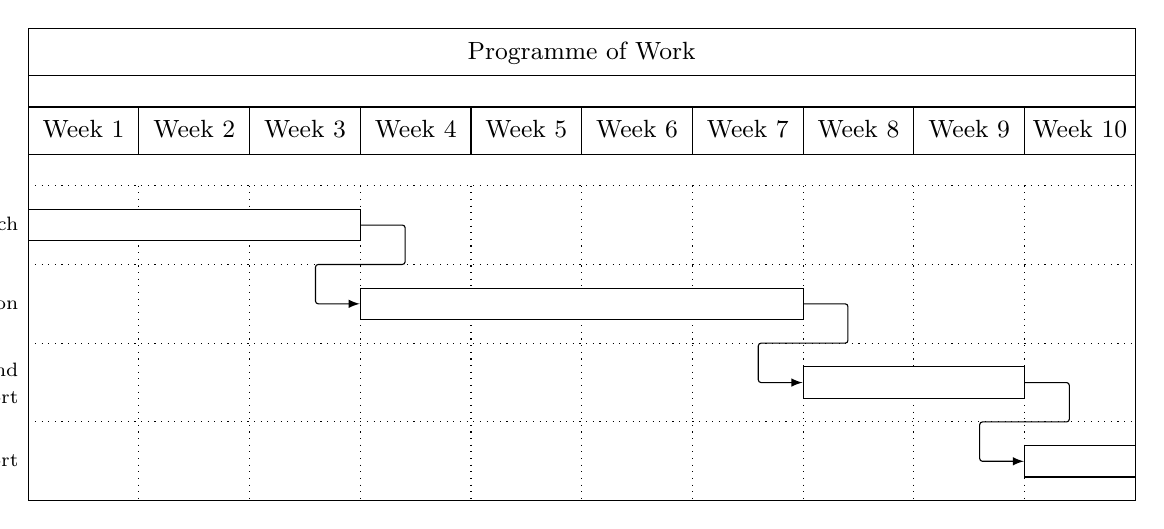
\begin{tikzpicture}
    \begin{pgfinterruptboundingbox}
      \begin{ganttchart}[canvas/.append style={alias=frame},
        hgrid, vgrid, x unit=4em,
        bar label node/.style={text width=3cm,align=right,font=\scriptsize\RaggedLeft,anchor=east}]{1}{10}
        
        \gantttitle{Programme of Work}{10} \\
        \gantttitlelist[title list options=%
        {var=\y, evaluate=\y as \x%
          using "Week \y"}]{1,...,10}{1} \\
        
        \ganttbar{Research}{1}{3}                           \\
        \ganttlinkedbar{OS Implementation}{4}{7}            \\
        \ganttlinkedbar{Testing and progress report}{8}{9}  \\
        \ganttlinkedbar{Progress report}{10}{10}                       
        
      \end{ganttchart}
    \end{pgfinterruptboundingbox}
    \useasboundingbox (frame.south west) rectangle (frame.north east);
  \end{tikzpicture}

  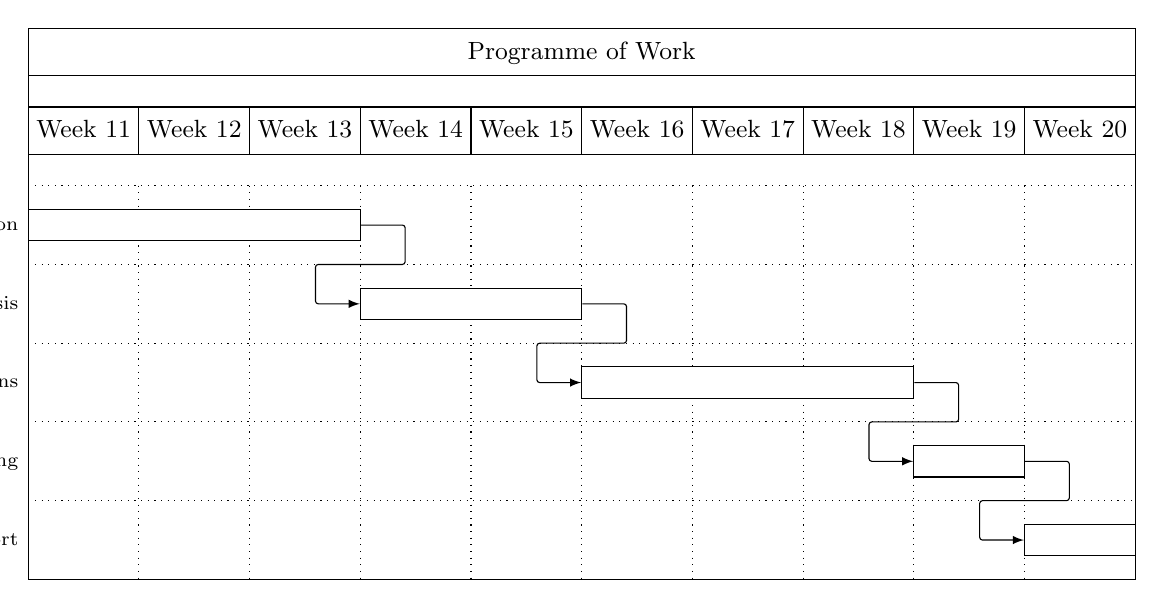
\begin{tikzpicture}
    \begin{pgfinterruptboundingbox}
      \begin{ganttchart}[canvas/.append style={alias=frame},
        hgrid, vgrid, x unit=4em,
        bar label node/.style={text width=3cm,align=right,font=\scriptsize\RaggedLeft,anchor=east}]{11}{20}
        
        \gantttitle{Programme of Work}{10} \\
        \gantttitlelist[title list options=%
        {var=\y, evaluate=\y as \x%
          using "Week \y"}]{11,...,20}{1} \\
        
        \ganttbar{Software Optimization}{11}{13}       \\
        \ganttlinkedbar{Performance Analysis}{14}{15}  \\
        \ganttlinkedbar{OS alterations}{16}{18}        \\
        \ganttlinkedbar{Final testing}{19}{19}         \\
        \ganttlinkedbar{Evaluation and Report}{20}{20}
        
      \end{ganttchart}
    \end{pgfinterruptboundingbox}
    \useasboundingbox (frame.south west) rectangle (frame.north east);
  \end{tikzpicture}

  \bibliographystyle{ieeetr}
  \bibliography{bib/proposal}
\end{document}